\documentclass{article}

% Import packages from local file
\usepackage{packages}

% Define the homework number as a variable
\newcommand{\HomeworkNumber}{7}

\begin{document}

% Add the cover


% Set up custom date format
\newdateformat{monthyeardate}{\monthname[\THEMONTH] \THEYEAR}

% Header and Footer configuration
\pagestyle{fancy}
\fancyhf{}
\fancyhead[L]{\leftmark}
\fancyhead[R]{\thepage}
\fancyfoot[C]{Probabilistic Modeling and Reasoning Homework \HomeworkNumber}

% Chapter and Section formatting
\titleformat{\chapter}[display]
  {\normalfont\bfseries}{}{0pt}{\Huge}
\titlespacing*{\chapter}{0pt}{-20pt}{20pt}

% Adjust header height and top margin
\setlength{\headheight}{14.49998pt}
\addtolength{\topmargin}{-2.49998pt}

% % Custom abstract environment
% \newenvironment{customabstract}
%   {\vspace*{1cm}
%    \begin{center}
%    \bfseries \huge Abstract
%    \end{center}
%    \vspace{0.5cm}
%    \normalfont \large}
%   {\vspace{1cm}}



\makeatletter
% Taken from http://ctan.org/pkg/centernot
\newcommand*{\centernot}{%
  \mathpalette\@centernot
}
\def\@centernot#1#2{%
  \mathrel{%
    \rlap{%
      \settowidth\dimen@{$\m@th#1{#2}$}%
      \kern.5\dimen@
      \settowidth\dimen@{$\m@th#1=$}%
      \kern-.5\dimen@
      $\m@th#1\not$%
    }%
    {#2}%
  }%
}
\makeatother


\begin{titlepage}
    \centering

    % University logo
    \vfill
    \includegraphics[width=0.3\textwidth]{UOMLOGOEN.eps}
    \vfill

    % Main title
    {\Huge \textbf{Probabilistic Modeling and Reasoning}} \\
    {\LARGE Homework — \HomeworkNumber}

    \vfill  % Vertical fill for dynamic centering
    % Authors' names
    {\Large \textbf{Nikolaos Liouliakis (AID25001)}} \\
    {\Large \textbf{Vasileios-Efraim Tsavalia (AID25006)}}

    % \vfill

    % % Course submission information
    % {\Large A report submitted for the course} \\
    % {\Large \textbf{Probabilistic Modeling and Reasoning}}

    \vfill

    % Program and University information
    {\Large MSc in Artificial Intelligence and Data Analytics} \\
    {\Large University of Macedonia}

    \vfill

    % Supervisor information
    {\Large \textbf{Supervisor: Professor Dimitris Christou-Varsakelis}}

    \vfill

    % Date with custom format
    {\Large \monthyeardate\today} % Automatically displays in "October 2024" format
    
\end{titlepage}


\newpage


\section*{Problem 1}

\subsection*{1. Show that \( p(f \mid \mathbf{x}) \) is Gaussian:}

We are given:
\[
f = \mathbf{w}^\top \mathbf{x}, \quad p(\mathbf{w}) \sim \mathcal{N}(\mathbf{w} \mid 0, \Sigma)
\]

Since \( f \) is a linear combination of the components of \( \mathbf{w} \), it is Gaussian. 
We only need to find its mean and variance:

The mean of \( f \):
\[
\mu_f = \mathbb{E}[f] = \mathbb{E}[\mathbf{w}^\top \mathbf{x}] = \mathbb{E}[\mathbf{w}]^\top \mathbf{x} = \mathbf{0}^\top \mathbf{x} = 0
\]

The variance of \( f \):
\[
\sigma_f^2 = \text{Var}(f) = \mathbb{E}[(f - \mu_f)^2] = \mathbb{E}[(\mathbf{w}^\top \mathbf{x})^2] 
= \mathbb{E}[\mathbf{w}^\top \mathbf{x}\mathbf{w}^\top \mathbf{x}] =
\]

\[
  \mathbb{E}[(\mathbf{w}^\top \mathbf{x})^\top \mathbf{w}^\top \mathbf{x}]
= \mathbb{E}[ \mathbf{x}^\top \mathbf{w} \mathbf{w}^\top \mathbf{x}]
= \mathbf{x}^\top \mathbb{E}[  \mathbf{w} \mathbf{w}^\top ] \mathbf{x}
= \mathbf{x}^\top \Sigma \mathbf{x}
\]

Thus:
\[
p(f \mid \mathbf{x}) = \mathcal{N}(f \mid 0, \mathbf{x}^\top \Sigma \mathbf{x})
\]


\subsection*{2. Find \( p(f \mid t, \mathbf{x}) \):}

We are given:
\[
t = f + \epsilon, \quad \epsilon \sim \mathcal{N}(0, \sigma^2)
\]

This implies:
\[
p(t \mid f) = \mathcal{N}(t \mid f, \sigma^2)
\]

The prior for \( f \):
\[
p(f \mid \mathbf{x}) = \mathcal{N}(f \mid 0, \mathbf{x}^\top \Sigma \mathbf{x})
\]

To compute \( p(f \mid t, \mathbf{x}) \), we use Bayes' theorem:
\[
p(f \mid t, \mathbf{x}) \propto p(t \mid f) p(f \mid \mathbf{x})
\]

Since both \( p(t \mid f) \) and \( p(f \mid \mathbf{x}) \) are Gaussian, their product results in another Gaussian distribution. The posterior mean and variance are derived using the standard formulas for combining Gaussians.

\textbf{Likelihood} \( p(t \mid f) \):
\[
p(t \mid f) = \frac{1}{\sqrt{2\pi \sigma^2}} \exp\left( -\frac{(t - f)^2}{2\sigma^2} \right)
\]

\textbf{Prior} \( p(f \mid \mathbf{x}) \):
\[
p(f \mid \mathbf{x}) = \frac{1}{\sqrt{2\pi \mathbf{x}^\top \Sigma \mathbf{x}}} \exp\left( -\frac{f^2}{2 \mathbf{x}^\top \Sigma \mathbf{x}} \right)
\]

\textbf{Posterior} \( p(f \mid t, \mathbf{x}) \):
The posterior is proportional to the product:
\[
p(f \mid t, \mathbf{x}) \propto \exp\left( -\frac{(t - f)^2}{2\sigma^2} - \frac{f^2}{2 \mathbf{x}^\top \Sigma \mathbf{x}} \right)
\]

Simplify the terms in the exponent:
\[
p(f \mid t, \mathbf{x}) \propto \exp\left(
% -\frac{(t - f)^2}{2\sigma^2} - \frac{f^2}{2 \mathbf{x}^\top \Sigma \mathbf{x}} = 
-\frac{t^2 - 2tf + f^2}{2\sigma^2} - \frac{f^2}{2 \mathbf{x}^\top \Sigma \mathbf{x}}
\right)
\]

\[
p(f \mid t, \mathbf{x}) \propto \exp\left(
-\frac{f^2}{2} \left( \frac{1}{\sigma^2} + \frac{1}{\mathbf{x}^\top \Sigma \mathbf{x}} \right)
+ f\frac{t}{\sigma^2}
- \frac{t^2}{2\sigma^2}
\right)
\]


\[
p(f \mid t, \mathbf{x}) \propto \exp\left(
-\frac{f^2}{2} \left( \frac{1}{\sigma^2} + \frac{1}{\mathbf{x}^\top \Sigma \mathbf{x}} \right)
+ f\frac{t}{\sigma^2}
% - \frac{t^2}{2\sigma^2}
\right)
\]

This is a Gaussian distribution with precision (inverse variance):
\[
\frac{1}{\sigma_{f \mid t}^2} = \frac{1}{\sigma^2} + \frac{1}{\mathbf{x}^\top \Sigma \mathbf{x}},
\]

variance:
\[
\sigma_{f \mid t}^2 = \left( \frac{1}{\sigma^2} + \frac{1}{\mathbf{x}^\top \Sigma \mathbf{x}} \right)^{-1} 
= \frac{\sigma^2 (\mathbf{x}^\top \Sigma \mathbf{x})}{\sigma^2 + \mathbf{x}^\top \Sigma \mathbf{x}},
\]

and mean:
\[
\mu_{f \mid t} =
\sigma_{f \mid t}^2 \frac{t}{\sigma^2}
=
\frac{\sigma^2 (\mathbf{x}^\top \Sigma \mathbf{x})}{\sigma^2 + \mathbf{x}^\top \Sigma \mathbf{x}} \frac{t}{\sigma^2}
% =
% \frac{\frac{t}{\sigma^2}}{\frac{1}{\sigma^2} + \frac{1}{\mathbf{x}^\top \Sigma \mathbf{x}}} 
= \frac{t \cdot (\mathbf{x}^\top \Sigma \mathbf{x})}{\sigma^2 + \mathbf{x}^\top \Sigma \mathbf{x}}
\]


Final Result:
\[
p(f \mid t, \mathbf{x}) = \mathcal{N}\left(f \mid \frac{t \cdot (\mathbf{x}^\top \Sigma \mathbf{x})}{\sigma^2 + \mathbf{x}^\top \Sigma \mathbf{x}}, \frac{\sigma^2 (\mathbf{x}^\top \Sigma \mathbf{x})}{\sigma^2 + \mathbf{x}^\top \Sigma \mathbf{x}} \right)
\]


\section*{Problem 2}

\textbf{Problem:}  
Show that for any integrable function \(f(\cdot)\), the following holds:  
\[
\int f(\mathbf{x}^\top \mathbf{w}) p(\mathbf{w}) d\mathbf{w} = \int f(h) p(h) dh
\]
% where:  
% - \(h = \mathbf{x}^\top \mathbf{w}\), and  
% - \(p(h)\) is the probability density function of the scalar random variable \(h\), defined as:
% \[
% p(h) = \int \delta(h - \mathbf{x}^\top \mathbf{w}) p(\mathbf{w}) d\mathbf{w}
% \]
% Here, \(p(\mathbf{w})\) is the probability density function of \(\mathbf{w}\), and \(\delta(\cdot)\) is the Dirac delta function.

% Assume that \(f(\cdot)\) is integrable and the necessary conditions for the use of the Dirac delta function and the change of variables in integration are satisfied.


\textbf{Proof:}

% \textit{Introduce the scalar \(h\):}  
Let \(h = \mathbf{x}^\top \mathbf{w}\), where \(\mathbf{w}\) is a vector and \(\mathbf{x}\) is a constant vector. By definition of \(p(h)\), it is the marginal distribution of \(h\) derived from the joint distribution of \(\mathbf{w}\). Specifically:
\[
p(h) = \int \delta(h - \mathbf{x}^\top \mathbf{w}) p(\mathbf{w}) d\mathbf{w}
\]
where \(\delta(\cdot)\) is the Dirac delta function

% \textit{Express the expectation over \(h\):}  
Using the definition of \(p(h)\), the integral over \(f(h)\) becomes:
\[
\int f(h) p(h) dh = \int f(h) \left( \int \delta(h - \mathbf{x}^\top \mathbf{w}) p(\mathbf{w}) d\mathbf{w} \right) dh
\]

% \textit{Switch the order of integration:}  
The order of integration can be swapped using Fubini’s theorem. Thus:
% because both \(h\) and \(\mathbf{w}\) are dummy variables. Thus:
\[
\int f(h) p(h) dh = \int \left( \int f(h) \delta(h - \mathbf{x}^\top \mathbf{w}) dh \right) p(\mathbf{w}) d\mathbf{w}
\]

% \textit{Evaluate the inner integral:}  
Using the property of the Dirac delta function, we have:

\[
\int f(h) \delta(h - \mathbf{x}^\top \mathbf{w}) dh = f(\mathbf{x}^\top \mathbf{w})
\]

% \textit{Substitute back into the integral:}  
Substituting this result into the equation gives:
\[
\int f(h) p(h) dh = \int f(\mathbf{x}^\top \mathbf{w}) p(\mathbf{w}) d\mathbf{w}
\]

% \textit{Conclusion:}  
% The left-hand side equals the right-hand side, proving the statement:
% \[
% \int f(\mathbf{x}^\top \mathbf{w}) p(\mathbf{w}) d\mathbf{w} = \int f(h) p(h) dh
% \]

\section*{Problem 3} 


We aim to derive the optimal regularization parameter \(\alpha\) for Bayesian Logistic Regression by maximizing the marginal log-likelihood \(L(\alpha)\), given as:
\[
L(\alpha) = -\frac{\alpha}{2} \mathbf{w}^\top \mathbf{w} + \sum_n \log \sigma((\mathbf{w}^\top \mathbf{h}^n)) - \frac{1}{2} \log \det (\alpha \mathbf{I} + \mathbf{J}) + \frac{B}{2} \log \alpha,
\]
where:
\begin{itemize}
    \item \(\mathbf{w}\) is the weight vector,
    \item \(\sigma(\cdot)\) is the sigmoid function,
    \item \(\mathbf{J}\) is the Hessian matrix of the negative log-likelihood with respect to \(\mathbf{w}\),
    \item \(B\) is the dimensionality of \(\mathbf{w}\).
\end{itemize}

\subsection*{Step 1: Total Derivative of \(L(\alpha)\)}

The total derivative of \(L(\alpha)\) with respect to \(\alpha\) is given by:
\[
\frac{dL}{d\alpha} = \frac{\partial L}{\partial \alpha} + \sum_i \frac{\partial L}{\partial w_i} \frac{\partial w_i}{\partial \alpha}.
\]

At the optimal \(\mathbf{w} = \mathbf{w}^*\), the gradient \(\frac{\partial L}{\partial \mathbf{w}} = 0\). Thus, the total derivative simplifies to:
\[
\frac{dL}{d\alpha} = \frac{\partial L}{\partial \alpha}.
\]

\subsection*{Step 2: Compute \(\frac{\partial L}{\partial \alpha}\)}

Using the expression for \(L(\alpha)\), we compute its derivative directly:
\[
\frac{\partial L}{\partial \alpha} = \frac{\partial}{\partial \alpha} \left( -\frac{\alpha}{2} \mathbf{w}^\top \mathbf{w} - \frac{1}{2} \log \det (\alpha \mathbf{I} + \mathbf{J}) + \frac{B}{2} \log \alpha \right).
\]

Taking the derivative term by term:

1. First term:
\[
\frac{\partial}{\partial \alpha} \left( -\frac{\alpha}{2} \mathbf{w}^\top \mathbf{w} \right) = -\frac{1}{2} \mathbf{w}^\top \mathbf{w}.
\]

2. Second term: For \(-\frac{1}{2} \log \det (\alpha \mathbf{I} + \mathbf{J})\), we use the identity:
\[
\frac{\partial}{\partial \alpha} \log \det (\mathbf{M}) = \text{trace} \left( \mathbf{M}^{-1} \frac{\partial \mathbf{M}}{\partial \alpha} \right),
\]
where \(\mathbf{M} = \alpha \mathbf{I} + \mathbf{J}\) and \(\frac{\partial \mathbf{M}}{\partial \alpha} = \mathbf{I}\). Therefore:
\[
\frac{\partial}{\partial \alpha} \left( -\frac{1}{2} \log \det (\alpha \mathbf{I} + \mathbf{J}) \right) = -\frac{1}{2} \text{trace} \left( (\alpha \mathbf{I} + \mathbf{J})^{-1} \right).
\]

3. Third term:
\[
\frac{\partial}{\partial \alpha} \left( \frac{B}{2} \log \alpha \right) = \frac{B}{2\alpha}.
\]

Combining these, the derivative is:
\[
\frac{\partial L}{\partial \alpha} = -\frac{1}{2} \mathbf{w}^\top \mathbf{w} - \frac{1}{2} \text{trace}((\alpha \mathbf{I} + \mathbf{J})^{-1}) + \frac{B}{2\alpha}.
\]

\subsection*{Step 3: Solve for \(\alpha\)}

To find the optimal \(\alpha\), set \(\frac{\partial L}{\partial \alpha} = 0\):
\[
-\frac{1}{2} \mathbf{w}^\top \mathbf{w} - \frac{1}{2} \text{trace}((\alpha \mathbf{I} + \mathbf{J})^{-1}) + \frac{B}{2\alpha} = 0.
\]

Multiply through by 2 to simplify:
\[
-\mathbf{w}^\top \mathbf{w} - \text{trace}((\alpha \mathbf{I} + \mathbf{J})^{-1}) + \frac{B}{\alpha} = 0.
\]

Rearranging:
\[
\frac{B}{\alpha} = \mathbf{w}^\top \mathbf{w} + \text{trace}((\alpha \mathbf{I} + \mathbf{J})^{-1}).
\]

% Finally, solving for \(\alpha\):
\[
\alpha = \frac{B}{\mathbf{w}^\top \mathbf{w} + \text{trace}((\alpha \mathbf{I} + \mathbf{J})^{-1})}.
\]

\subsection*{Step 4: Fixed-Point Equation}

After substituting $ \mathbf{w}$ with $ \mathbf{w}^*$, the fixed-point equation for \(\alpha\) is:
\[
\alpha^{\text{new}} = \frac{B}{\mathbf{w}^{*\top} \mathbf{w}^* + \text{trace}((\alpha \mathbf{I} + \mathbf{J})^{-1})}.
\]


\section*{Problem 4}

The file \textit{HW7\_P4\_main.m} implements the main functionality.
For the estimation of the $a$ and $b$ hyperparameters the Gull-MacKay fixed point iteration method was used.


\begin{figure}[H]
    \centering
    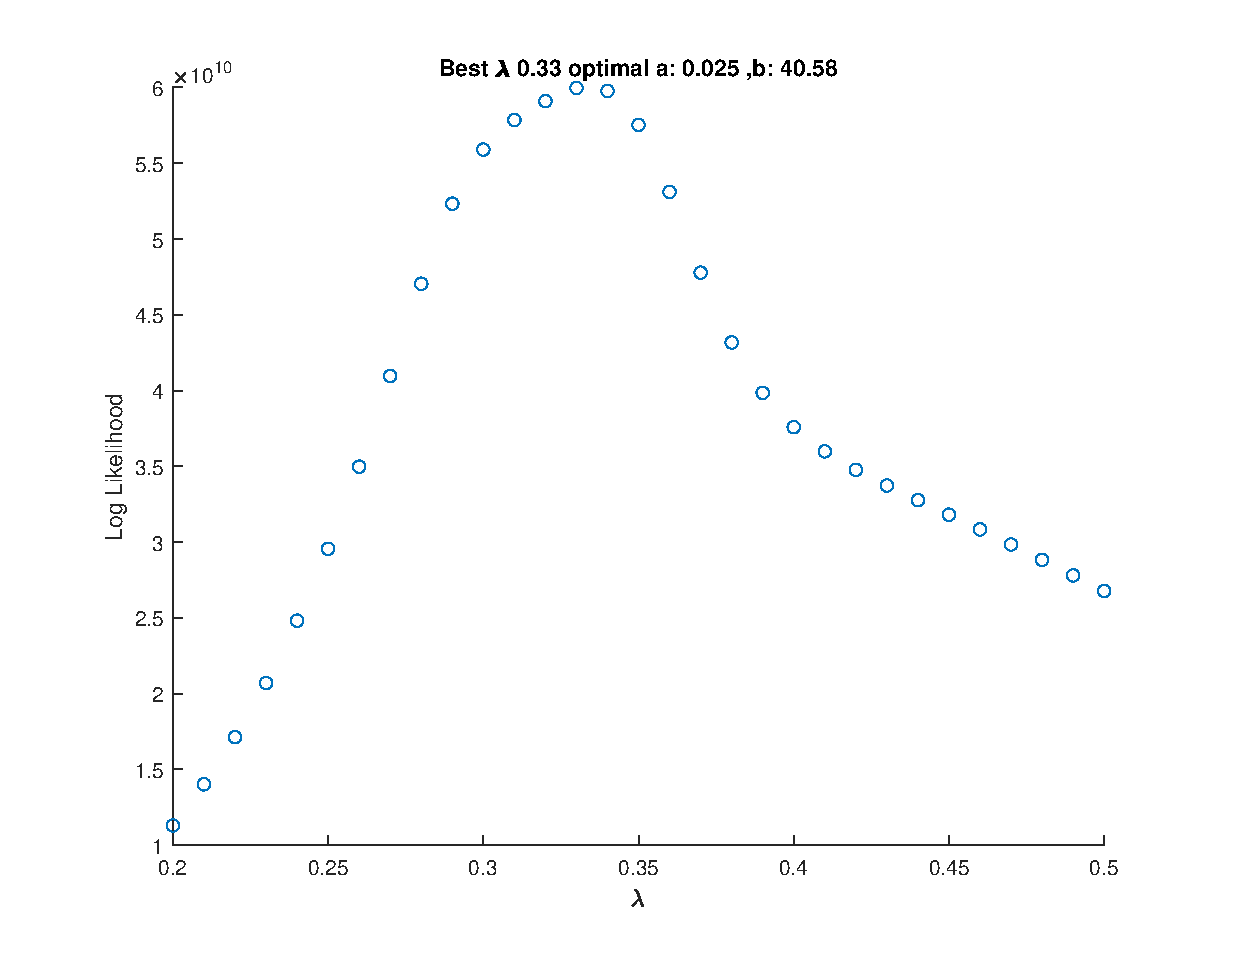
\includegraphics[width=\textwidth]{log_like_lambda.eps}     
    \caption{The log marginal likelihood for various $\lambda$.}
\end{figure}



\begin{figure}[H]
    \centering
    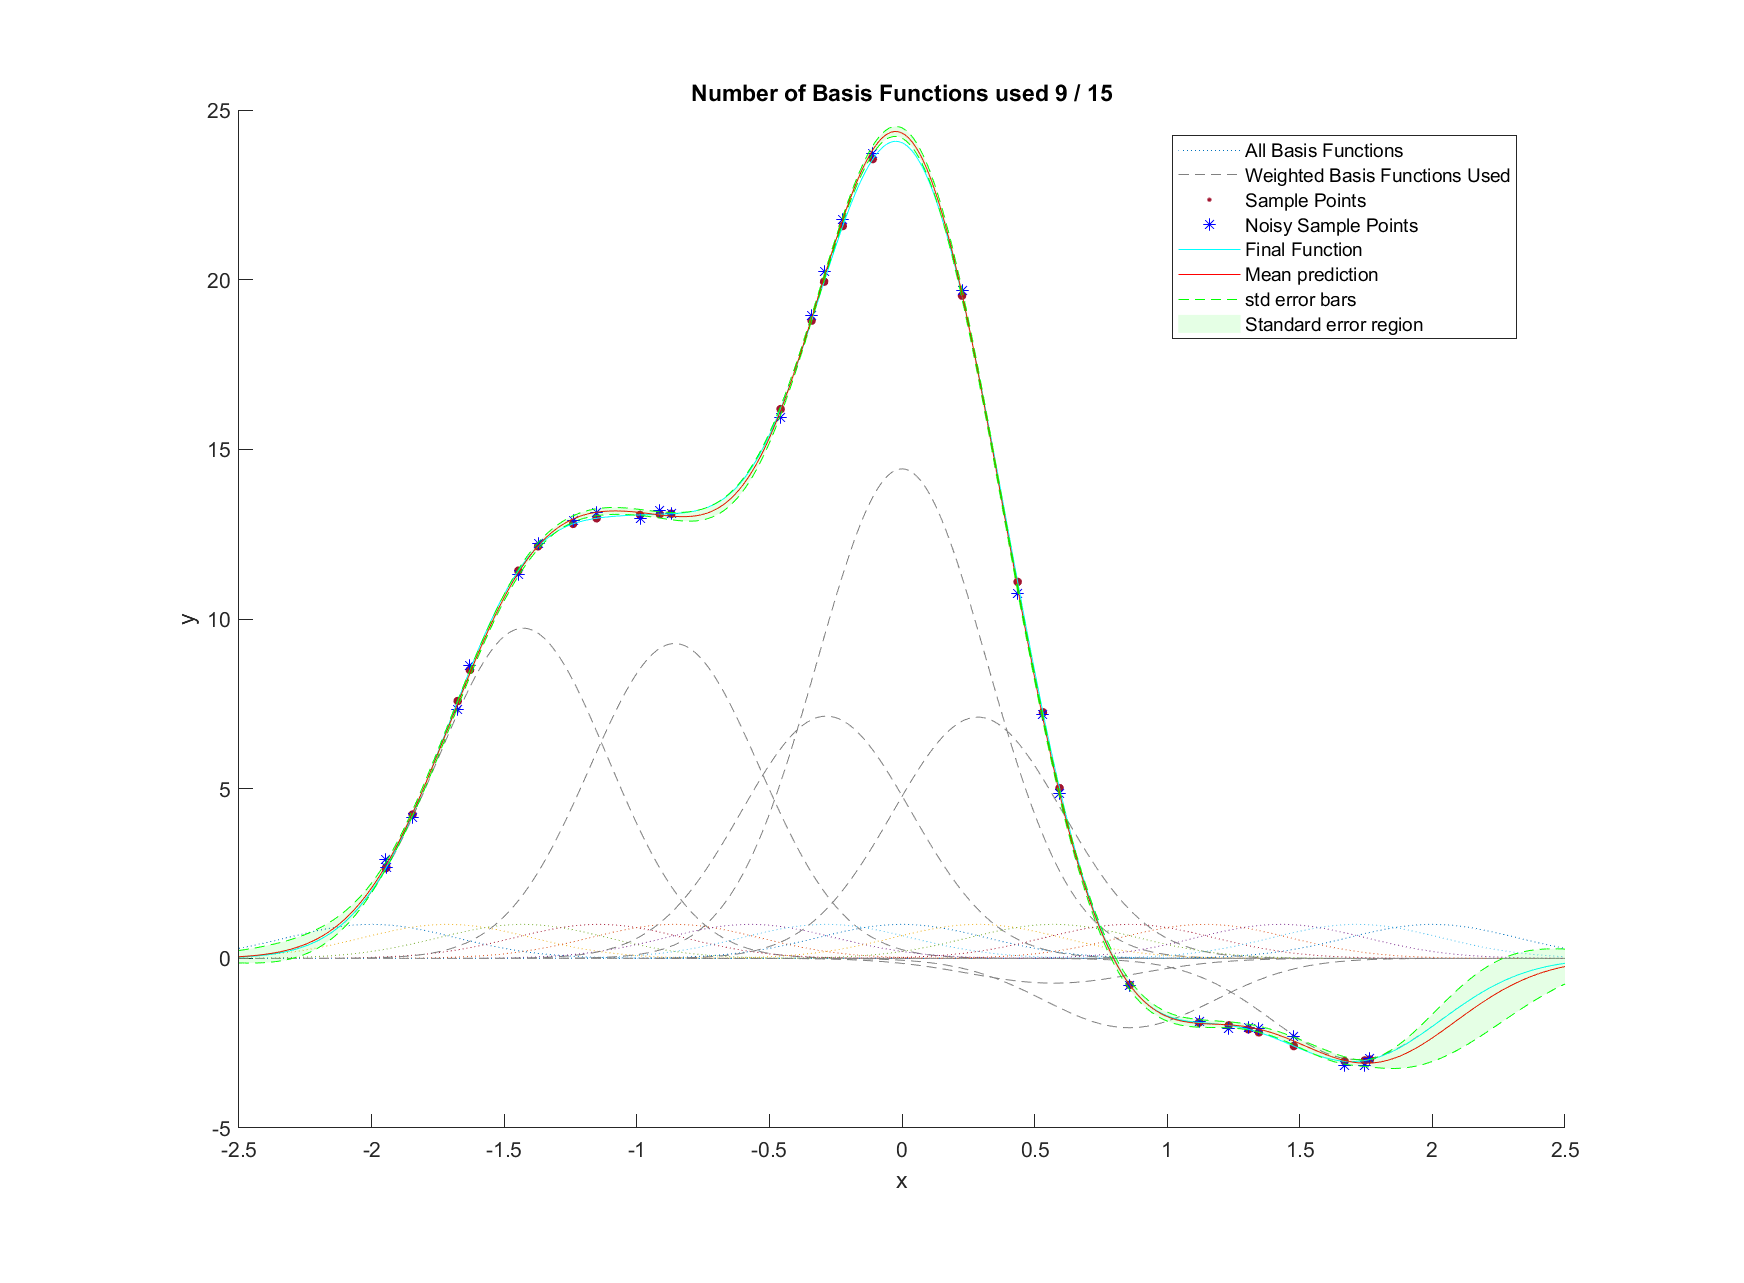
\includegraphics[width=\textwidth]{points_and_curves.eps}     
    \caption{Training data points and the predicted
curve with error bars.}
\end{figure}



\end{document}
